\qs{}{
    What is the average high school grade for each school?
}

Calculate the average high school grade for each school by selecting \texttt{DISTINCT} school names from the \texttt{student} table. Compute the average of high school grades associated with each school using \texttt{AVG()}. Sort the results in descending order based on the average high school grade using \texttt{DESC}.
\vspace{\baselineskip}


\sol{}
\noindent\line(1, 0){0.89\linewidth}
\begin{verbatim}
SELECT stud_hs_name AS school_name, AVG(stud_hs_grade) AS average_high_school_grade
FROM student
WHERE stud_hs_name IS NOT NULL
GROUP BY stud_hs_name
ORDER BY average_high_school_grade DESC;
\end{verbatim}
\noindent\line(1, 0){\linewidth}

\begin{figure}[H]
    \centering
    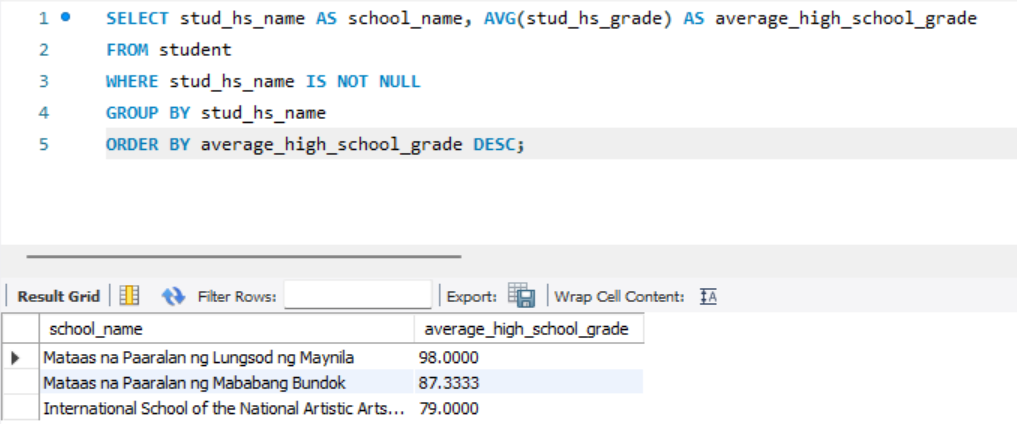
\includegraphics[width=0.7\linewidth]{images/q12.png}
    \caption{Question 12 Query and Output}
\end{figure}
